\section{Posture recognition}
As suggested by \cite{orientation}, since we analyze the hand frame by frame instead of analyzing it over a time period, we would call the information  ``posture'' instead of ``gesture'', which suggests a movement. The problem we would like to solve here is, given the input image, we want to decide which posture the hand in the image poses. As a matter of fact, this is a classic classification problem in the machine learning literature, so we choose to solve this with a machine learning approach. It is possible to come up with another way to deal with this problem, for example one could give a clear difinition for each of the postures. However, one would have to do this for each postures used in the system. Thus, for generality, although our system only utilizes two postures, we will still solve it with a machine learning technique. 

The algorithm we use is the k-nearest neighbors algorithm. Simply put, this algorithm finds the $k$ images in a database that are the ``nearest'' to the image to be classified, then classifies it as the most common posture among the $k$ neighbors. The ``similarity'' between the images should be properly defined to reflect the nature of the images and the postures. The problem then is how we should define the similarity. 

Because we are only classifying the hand posture, the other informations in the image are unnecessary. Thus for each image we first apply the hand detection algorithm to find the area of the hand, then we discard all the pixels that are deemed not to be hand. We can then calculate the orientation histogram of the hand. That is, we calculate the gradient orientation of each pixel, defined as
\begin{align}
arctan(dx, dy)
\end{align}•
where $dx$, $dy$ are the image gradient of the pixel. However, since the image $img(x,y)$ is a discrete function, instead of the gradient, we can only compute an approximate of it. The approximation we choose is the Sobel operator. The Sobel operator, in its simplest case, basically has two kernels: one for horizontal gradient and one for vertical gradient. The kernels are 
\begin{align*}
 G_x(Img) = 
 \left[
  \begin{tabular}{c c c}
   -1&0&+1\\
   -2&0&+2\\
   -1&0&+1\\
  \end{tabular}
 \right]
*Img\\
G_y(Img) =
\left[
\begin{tabular}{c c c}
-1&-2&+1\\
0&0&0\\
-1&-2&+1\\
\end{tabular}
\right]
*Img\\
\end{align*}
, where $Img$ is the input image, and $*$ symbol is the 2-D convolution. 

After we compute the orientation of each pixel, we put it into one of the $36$ bins. The $i$th bin is $[-\pi+(i-1)\pi/18, -\pi+i\pi/18)$. Thus, we will have an orientation histogram of length $36$. This vector can serve as our feature for the image. 

Since the same hand posture can have different orientation, we can furthur reduce the intrinsic dimension of the feature by rotating the image. We assume that when the user makes the same posture with different orientations, the orientation histograms will have the same distribution, but will have a disposition. Thus, if we rotate the image so that the hand in the two image have the same orientation, their orientation histogram should be similar. This can be done by finding the major axis of the hand, then, instead of rotate the image before computing the orientation histogram, we can simply translate the orientation histogram by the angle of the major axis. As can be shown in Fig. \ref{fig:or_hist}, this method does give us a histogram that is distinctive with respect to the hand posture, and insensitive to the orientation of the hand. 
\begin{figure}
\begin{tabular}{lll}
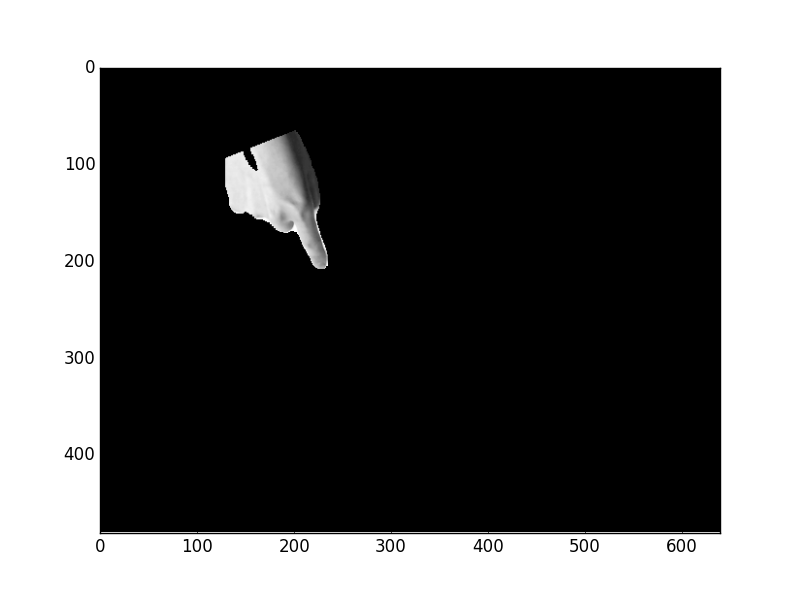
\includegraphics[width=4cm]{fig8/gray_550.png} &
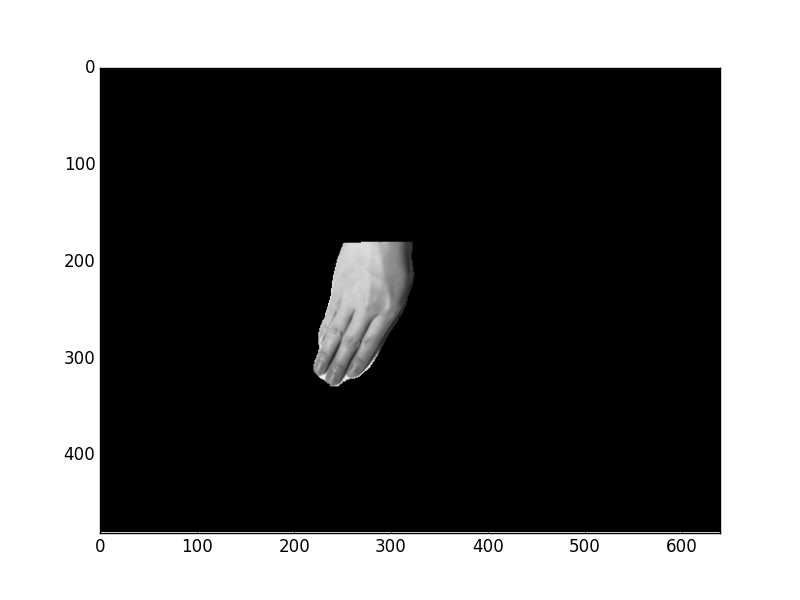
\includegraphics[width=4cm]{fig8/gray_341.png} &
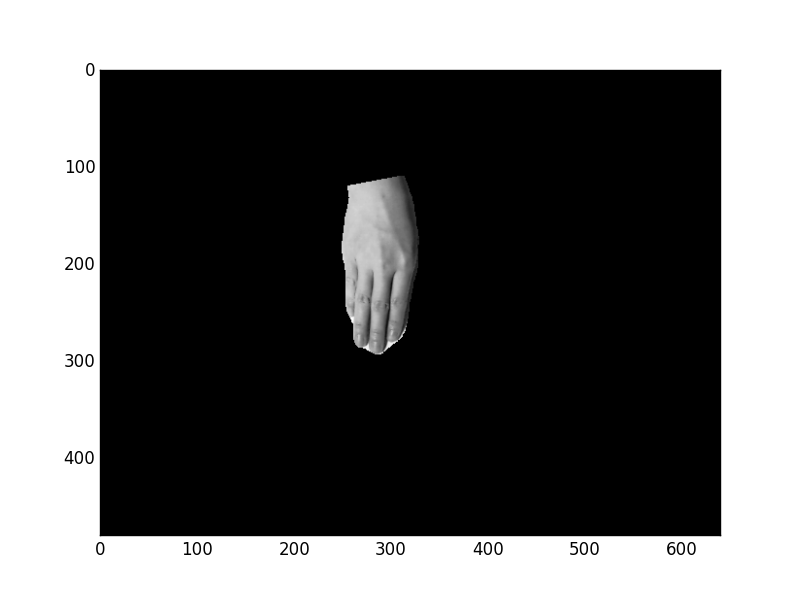
\includegraphics[width=4cm]{fig8/gray_318.png} \\
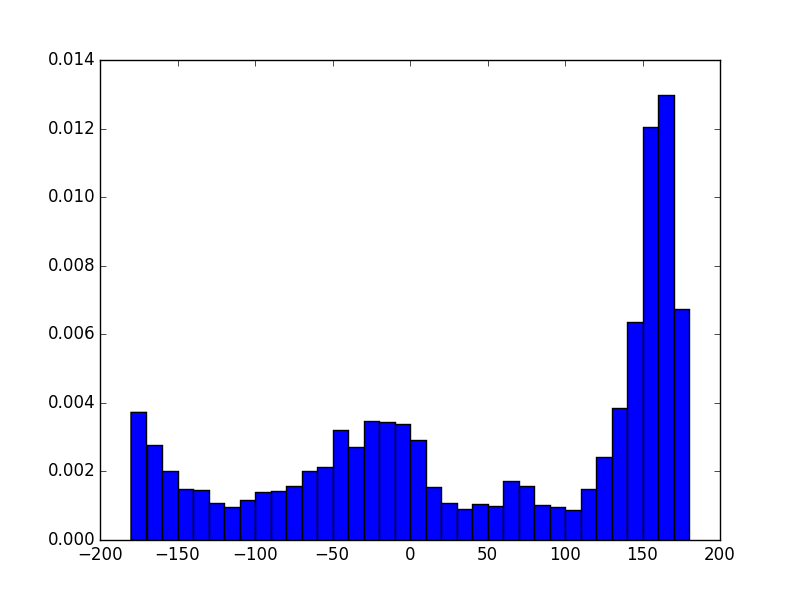
\includegraphics[width=4cm]{fig8/figure_550.png} &
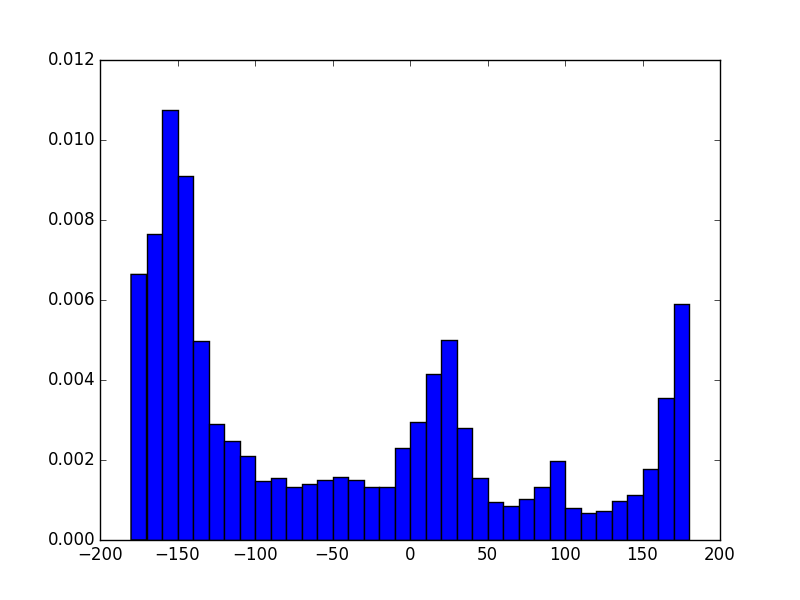
\includegraphics[width=4cm]{fig8/hist_341.png} &
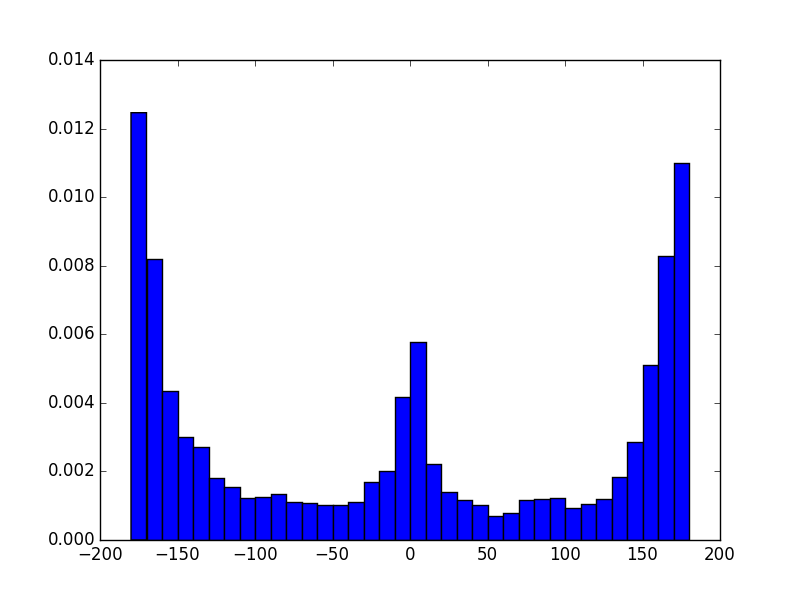
\includegraphics[width=4cm]{fig8/hist_318.png} \\
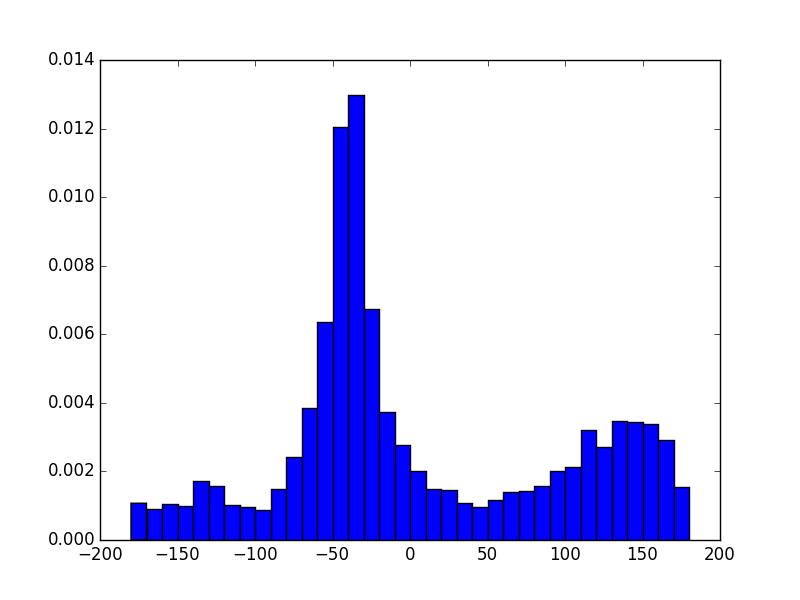
\includegraphics[width=4cm]{fig8/figure_550_t.png} &
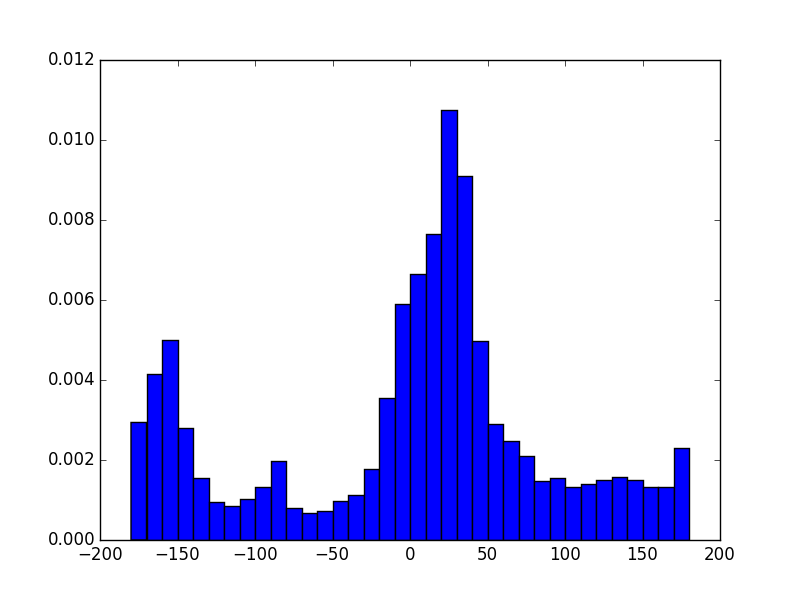
\includegraphics[width=4cm]{fig8/hist_341_t.png} &
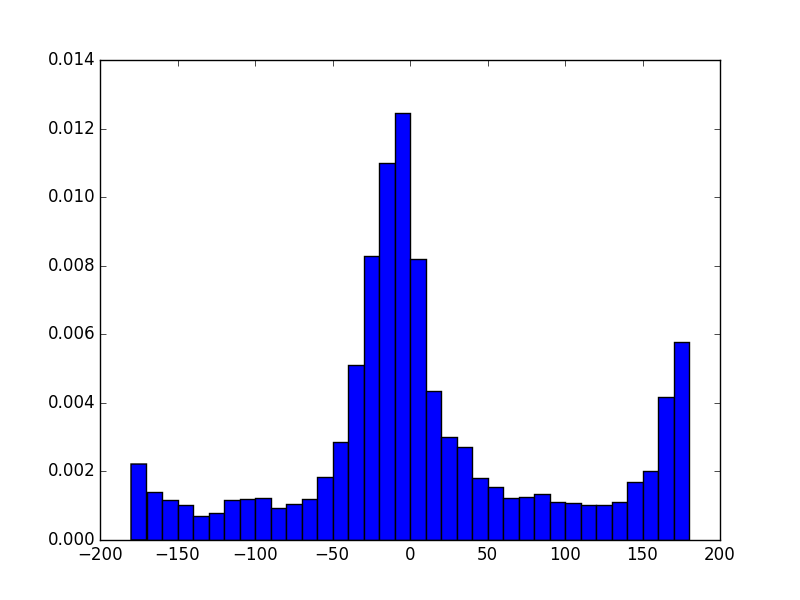
\includegraphics[width=4cm]{fig8/hist_318_t.png}
\end{tabular}

\caption{The orientation histograms. The first row is the input image, converted to gray scale and applied hand detection. The second row is the orientation histogram. The third row is the orientation histogram after the translation of the major axis.}
\label{fig:or_hist}
\end{figure}•

